% Algebra 2 Lesson 3-5 fast-track packet: Zeros of Polynomial Functions
% (enVision A2 2024 TE, Example 1 and Example 2 only; Examples 3-6 cut, fast-lesson spec R1-R3).
% Quiz items fed: 1 (Part A zeros, Part B sketch) by Example 1; 4 and 5 (multiplicity, behavior at each zero) by Example 2.
% Shared preamble for the "fast" (hacked-down) Algebra 2 lesson packets, Oct 2026.
% Each packet: % Shared preamble for the "fast" (hacked-down) Algebra 2 lesson packets, Oct 2026.
% Each packet: % Shared preamble for the "fast" (hacked-down) Algebra 2 lesson packets, Oct 2026.
% Each packet: \input{fast-packet-template} then \begin{document} ... \end{document}.
\documentclass[12pt]{article}
\usepackage[margin=0.7in]{geometry}
\usepackage{amsmath,amssymb}
\usepackage{booktabs,tabularx,array}
\usepackage{enumitem}
\usepackage[T1]{fontenc}
\usepackage[utf8]{inputenc}
\usepackage{lmodern}
\usepackage{tikz}
\usepackage{pgfplots}
\pgfplotsset{compat=1.18}
\usepackage{xcolor}
\setlist{nosep,leftmargin=1.4em}
\setlength{\parindent}{0pt}
\setlength{\parskip}{6pt}
\renewcommand{\arraystretch}{1.35}
\newcolumntype{Y}{>{\raggedright\arraybackslash}X}
\pagestyle{empty}

% blanks and workspace
\newcommand{\blank}[1][2.6cm]{\rule[-2pt]{#1}{0.5pt}}
\newcommand{\lines}[1][1]{\par\vspace{2pt}\foreach \i in {1,...,#1}{\rule{0pt}{22pt}\rule{\linewidth}{0.4pt}\par}}
\newcommand{\wspart}[2]{\vspace{4pt}{\large\bfseries #1: #2}\par\vspace{-6pt}\rule{\textwidth}{0.4pt}\par}

% header: \packethead{Lesson 1-3}{Piecewise-Defined Functions}
\newcommand{\packethead}[2]{%
{\LARGE\bfseries #2}\hfill Name \blank[5cm]\\[2pt]
Algebra 2 \quad #1 (fast track) \hfill Date \blank[2.5cm] \quad Period \blank[1.2cm]\par\vspace{2pt}}

% boxed goals: \goals{learning goal}{language goal}
\newcommand{\goals}[2]{%
\fbox{\parbox{\dimexpr\textwidth-2\fboxsep-2\fboxrule}{%
\textbf{Learning goal:} #1\\[2pt]
\textbf{Language goal:} #2}}\par}

% quiz target box: \quiztarget{text}
\newcommand{\quiztarget}[1]{%
\vspace{4pt}\colorbox{gray!12}{\parbox{\dimexpr\textwidth-2\fboxsep}{\textbf{On the quiz:} #1}}\par}

% IXL table row helper: code & skill & which quiz question it feeds
\newcommand{\ixlrow}[3]{\texttt{#1} & #2 & #3 \\}

% one grid style for every graph; override xmin/xmax/... per plot
\pgfplotsset{sheetgrid/.style={
  axis lines=middle, grid=both, grid style={gray!45},
  xmin=-10.5, xmax=10.5, ymin=-10.5, ymax=10.5,
  xtick={-10,-8,...,10}, ytick={-10,-8,...,10},
  x=0.28cm, y=0.28cm,
  ticklabel style={font=\scriptsize, fill=white, inner sep=1pt},
  xlabel={$x$}, ylabel={$y$},
  axis line style={thick}, clip=true}}
% unit grid for small windows
\pgfplotsset{unitgrid/.style={sheetgrid,
  xmin=-5.5, xmax=5.5, ymin=-5.5, ymax=5.5,
  xtick={-5,...,5}, ytick={-5,...,5}, x=0.5cm, y=0.5cm}}
% open and closed endpoints
\tikzset{closed/.style={circle, fill, inner sep=1.6pt},
         open/.style={circle, draw, fill=white, inner sep=1.4pt}}
 then \begin{document} ... \end{document}.
\documentclass[12pt]{article}
\usepackage[margin=0.7in]{geometry}
\usepackage{amsmath,amssymb}
\usepackage{booktabs,tabularx,array}
\usepackage{enumitem}
\usepackage[T1]{fontenc}
\usepackage[utf8]{inputenc}
\usepackage{lmodern}
\usepackage{tikz}
\usepackage{pgfplots}
\pgfplotsset{compat=1.18}
\usepackage{xcolor}
\setlist{nosep,leftmargin=1.4em}
\setlength{\parindent}{0pt}
\setlength{\parskip}{6pt}
\renewcommand{\arraystretch}{1.35}
\newcolumntype{Y}{>{\raggedright\arraybackslash}X}
\pagestyle{empty}

% blanks and workspace
\newcommand{\blank}[1][2.6cm]{\rule[-2pt]{#1}{0.5pt}}
\newcommand{\lines}[1][1]{\par\vspace{2pt}\foreach \i in {1,...,#1}{\rule{0pt}{22pt}\rule{\linewidth}{0.4pt}\par}}
\newcommand{\wspart}[2]{\vspace{4pt}{\large\bfseries #1: #2}\par\vspace{-6pt}\rule{\textwidth}{0.4pt}\par}

% header: \packethead{Lesson 1-3}{Piecewise-Defined Functions}
\newcommand{\packethead}[2]{%
{\LARGE\bfseries #2}\hfill Name \blank[5cm]\\[2pt]
Algebra 2 \quad #1 (fast track) \hfill Date \blank[2.5cm] \quad Period \blank[1.2cm]\par\vspace{2pt}}

% boxed goals: \goals{learning goal}{language goal}
\newcommand{\goals}[2]{%
\fbox{\parbox{\dimexpr\textwidth-2\fboxsep-2\fboxrule}{%
\textbf{Learning goal:} #1\\[2pt]
\textbf{Language goal:} #2}}\par}

% quiz target box: \quiztarget{text}
\newcommand{\quiztarget}[1]{%
\vspace{4pt}\colorbox{gray!12}{\parbox{\dimexpr\textwidth-2\fboxsep}{\textbf{On the quiz:} #1}}\par}

% IXL table row helper: code & skill & which quiz question it feeds
\newcommand{\ixlrow}[3]{\texttt{#1} & #2 & #3 \\}

% one grid style for every graph; override xmin/xmax/... per plot
\pgfplotsset{sheetgrid/.style={
  axis lines=middle, grid=both, grid style={gray!45},
  xmin=-10.5, xmax=10.5, ymin=-10.5, ymax=10.5,
  xtick={-10,-8,...,10}, ytick={-10,-8,...,10},
  x=0.28cm, y=0.28cm,
  ticklabel style={font=\scriptsize, fill=white, inner sep=1pt},
  xlabel={$x$}, ylabel={$y$},
  axis line style={thick}, clip=true}}
% unit grid for small windows
\pgfplotsset{unitgrid/.style={sheetgrid,
  xmin=-5.5, xmax=5.5, ymin=-5.5, ymax=5.5,
  xtick={-5,...,5}, ytick={-5,...,5}, x=0.5cm, y=0.5cm}}
% open and closed endpoints
\tikzset{closed/.style={circle, fill, inner sep=1.6pt},
         open/.style={circle, draw, fill=white, inner sep=1.4pt}}
 then \begin{document} ... \end{document}.
\documentclass[12pt]{article}
\usepackage[margin=0.7in]{geometry}
\usepackage{amsmath,amssymb}
\usepackage{booktabs,tabularx,array}
\usepackage{enumitem}
\usepackage[T1]{fontenc}
\usepackage[utf8]{inputenc}
\usepackage{lmodern}
\usepackage{tikz}
\usepackage{pgfplots}
\pgfplotsset{compat=1.18}
\usepackage{xcolor}
\setlist{nosep,leftmargin=1.4em}
\setlength{\parindent}{0pt}
\setlength{\parskip}{6pt}
\renewcommand{\arraystretch}{1.35}
\newcolumntype{Y}{>{\raggedright\arraybackslash}X}
\pagestyle{empty}

% blanks and workspace
\newcommand{\blank}[1][2.6cm]{\rule[-2pt]{#1}{0.5pt}}
\newcommand{\lines}[1][1]{\par\vspace{2pt}\foreach \i in {1,...,#1}{\rule{0pt}{22pt}\rule{\linewidth}{0.4pt}\par}}
\newcommand{\wspart}[2]{\vspace{4pt}{\large\bfseries #1: #2}\par\vspace{-6pt}\rule{\textwidth}{0.4pt}\par}

% header: \packethead{Lesson 1-3}{Piecewise-Defined Functions}
\newcommand{\packethead}[2]{%
{\LARGE\bfseries #2}\hfill Name \blank[5cm]\\[2pt]
Algebra 2 \quad #1 (fast track) \hfill Date \blank[2.5cm] \quad Period \blank[1.2cm]\par\vspace{2pt}}

% boxed goals: \goals{learning goal}{language goal}
\newcommand{\goals}[2]{%
\fbox{\parbox{\dimexpr\textwidth-2\fboxsep-2\fboxrule}{%
\textbf{Learning goal:} #1\\[2pt]
\textbf{Language goal:} #2}}\par}

% quiz target box: \quiztarget{text}
\newcommand{\quiztarget}[1]{%
\vspace{4pt}\colorbox{gray!12}{\parbox{\dimexpr\textwidth-2\fboxsep}{\textbf{On the quiz:} #1}}\par}

% IXL table row helper: code & skill & which quiz question it feeds
\newcommand{\ixlrow}[3]{\texttt{#1} & #2 & #3 \\}

% one grid style for every graph; override xmin/xmax/... per plot
\pgfplotsset{sheetgrid/.style={
  axis lines=middle, grid=both, grid style={gray!45},
  xmin=-10.5, xmax=10.5, ymin=-10.5, ymax=10.5,
  xtick={-10,-8,...,10}, ytick={-10,-8,...,10},
  x=0.28cm, y=0.28cm,
  ticklabel style={font=\scriptsize, fill=white, inner sep=1pt},
  xlabel={$x$}, ylabel={$y$},
  axis line style={thick}, clip=true}}
% unit grid for small windows
\pgfplotsset{unitgrid/.style={sheetgrid,
  xmin=-5.5, xmax=5.5, ymin=-5.5, ymax=5.5,
  xtick={-5,...,5}, ytick={-5,...,5}, x=0.5cm, y=0.5cm}}
% open and closed endpoints
\tikzset{closed/.style={circle, fill, inner sep=1.6pt},
         open/.style={circle, draw, fill=white, inner sep=1.4pt}}

\begin{document}

\packethead{Lesson 3-5}{Zeros of Polynomial Functions}
\goals{I can find the zeros of a polynomial function by factoring and use them to sketch its graph.}{I can explain what a graph does at each zero using the words zero, factor, multiplicity, crosses, and turning point.}

\quiztarget{(1) Factor a cubic, list all its zeros, and sketch its graph through them (Example 1). (2) Solve a polynomial equation (full Savvas quiz only). (3) Solve a polynomial inequality (full Savvas quiz only). (4) Read the zeros and their multiplicities off a graph (Example 2). (5) Find the zeros of a cubic with a double zero and pick the right description of its graph: end behavior, above or below the $x$-axis between zeros, where it touches the axis (Examples 1 and 2, then the Practice).}
\topictarget{3}{Question 11: does $f(x)=(x-5)(x-1)(x+4)$ cross or touch the $x$-axis at each zero (Example 2)? Question 12: the zeros of $f(x)=x(x-3)(x+1)$ (Example 1).}

\wspart{Example 1}{Use Zeros to Graph a Polynomial Function}
What are the zeros of $f(x)=x(x-4)(x+3)$? Graph the function.

\begin{minipage}[t]{0.55\textwidth}
\vspace{0pt}
\textbf{1. Zeros.} A \textbf{zero} is an $x$-value where $f(x)=0$. By the Zero-Product Property, a product is 0 only when a \textbf{factor} is 0:
\[x=0 \qquad x-4=0\Rightarrow x=4 \qquad x+3=0\Rightarrow x=-3\]
The zeros are $-3$, $0$ and $4$.

\textbf{2. Intervals.} The zeros cut the number line into four intervals.

\begin{center}
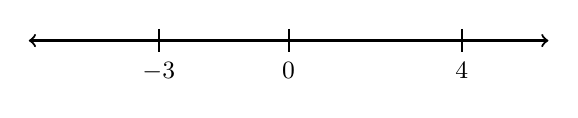
\begin{tikzpicture}[x=0.55cm]
\draw[<->, thick] (-6,0) -- (6,0);
\foreach \t in {-3,0,4} {\draw[thick] (\t,0.15) -- (\t,-0.15); \node[below, font=\small] at (\t,-0.15) {$\t$};}
\end{tikzpicture}
\end{center}

\textbf{3. Signs.} Pick the sign of each factor on each interval; the product's sign says where the graph is.

\small
\begin{tabular}{|l|c|c|c|c|l|}
\hline
\textbf{Interval} & $x$ & $x-4$ & $x+3$ & \textbf{Product} & \textbf{Graph} \\ \hline
$x<-3$ & $-$ & $-$ & $-$ & $-$ & below \\
$-3<x<0$ & $-$ & $-$ & $+$ & $+$ & above \\
$0<x<4$ & $+$ & $-$ & $+$ & $-$ & below \\
$x>4$ & $+$ & $+$ & $+$ & $+$ & above \\ \hline
\end{tabular}
\normalsize
\end{minipage}\hfill
\begin{minipage}[t]{0.42\textwidth}
\vspace{0pt}
\textbf{4. Sketch.} Draw one smooth curve through each zero: below the $x$-axis where the product is negative, above it where the product is positive.

\begin{center}
\begin{tikzpicture}
\begin{axis}[sheetgrid, xmin=-6.5, xmax=6.5, ymin=-25, ymax=25,
  xtick={-6,-4,-2,2,4,6}, xticklabels={$-6$,$-4$,$-2$,$2$,,$6$},
  ytick={-20,-10,...,20}, minor xtick={-6,...,6},
  x=0.5cm, y=0.13cm]
\addplot[very thick, blue, domain=-3.85:4.7, samples=120] {x*(x-4)*(x+3)};
\node[closed] at (axis cs:-3,0) {};
\node[closed] at (axis cs:0,0) {};
\node[closed] at (axis cs:4,0) {};
\node[font=\scriptsize, fill=white, inner sep=1pt, anchor=north west] at (axis cs:4.05,-0.9) {$4$};
\node[font=\scriptsize, blue, fill=white, inner sep=1pt] at (axis cs:3.6,18) {$f$};
\node[font=\scriptsize, fill=white, inner sep=0.5pt, anchor=north east] at (axis cs:-0.15,-0.8) {$O$};
\end{axis}
\end{tikzpicture}
\end{center}
\small Check: $f(-2)=(-2)(-6)(1)=12$ and $f(2)=(2)(-2)(5)=-20$, so the curve really is above, then below.
\end{minipage}

\vspace{4pt}
\textbf{Say it:} The \textbf{zeros} of $f$ are \blank[2.6cm] because each \textbf{factor} \blank[3.6cm]. On \mbox{$-3<x<0$} the graph is \blank[2cm] the $x$-axis because \blank[5cm].
\lines[1]

\newpage
\wspart{Try It 1}{Factor each function. Then use the zeros to sketch its graph.}
\begin{minipage}[t]{0.48\textwidth}
\vspace{0pt}
\textbf{a.} $f(x)=4x^3+4x^2-24x$

\vspace{2pt}
Factor: $f(x)=\blank[4.5cm]$

Zeros: \blank[4.5cm]
\begin{center}
\begin{tikzpicture}
\begin{axis}[sheetgrid, xmin=-5.5, xmax=5.5, ymin=-45, ymax=45,
  xtick={-5,...,5}, ytick={-40,-30,...,40}, x=0.55cm, y=0.058cm,
  ticklabel style={font=\tiny, fill=white, inner sep=0.5pt}]
\node[font=\tiny, fill=white, inner sep=0.5pt, anchor=south east] at (axis cs:-0.08,1.5) {$O$};
\end{axis}
\end{tikzpicture}
\end{center}
\end{minipage}\hfill
\begin{minipage}[t]{0.48\textwidth}
\vspace{0pt}
\textbf{b.} $g(x)=x^4-81$

Hint: $x^4-81=(x^2)^2-9^2$; the factor $x^2+9$ is never 0 for a real $x$.

\vspace{2pt}
Factor: $g(x)=\blank[4.5cm]$

Zeros: \blank[4.5cm]
\begin{center}
\begin{tikzpicture}
\begin{axis}[sheetgrid, xmin=-5.5, xmax=5.5, ymin=-100, ymax=60,
  xtick={-5,...,5}, ytick={-100,-80,...,60}, x=0.55cm, y=0.033cm,
  ticklabel style={font=\tiny, fill=white, inner sep=0.5pt}]
\node[font=\tiny, fill=white, inner sep=0.5pt, anchor=south east] at (axis cs:-0.08,2.5) {$O$};
\end{axis}
\end{tikzpicture}
\end{center}
\end{minipage}

Sign table for part a (one row per interval):\par\vspace{-4pt}
\renewcommand{\arraystretch}{1.25}
\begin{tabular}{|p{3cm}|p{2.2cm}|p{2.2cm}|p{2.2cm}|p{2cm}|p{2.2cm}|}
\hline
\textbf{Interval} & \textbf{factor} & \textbf{factor} & \textbf{factor} & \textbf{Product} & \textbf{Graph} \\ \hline
 & & & & & \\ \hline
 & & & & & \\ \hline
 & & & & & \\ \hline
 & & & & & \\ \hline
\end{tabular}

\renewcommand{\arraystretch}{1.35}

\wspart{Extension}{Practice 30 (DOK 3), when you finish}
\textbf{Performance Task} Venetta opened several deli sandwich franchises in 2000. The profit $P$ (in hundreds of dollars) of the franchises in $t$ years (since the franchises opened) can be modeled by the function $P(t)=t^3+t^2-6t$.

\begin{minipage}[t]{0.42\textwidth}
\vspace{0pt}
\textbf{Part A} Sketch a graph of the function.

\begin{tikzpicture}
\begin{axis}[sheetgrid, xmin=-1, xmax=25.5, ymin=-2000, ymax=17000,
  xtick={0,6,...,24}, ytick={4000,8000,...,16000}, minor x tick num=1, minor y tick num=1,
  minor grid style={gray!25}, x=0.22cm, y=0.0002cm, xlabel={$t$}, ylabel={$P$},
  scaled y ticks=false, yticklabel={\pgfmathprintnumber[set thousands separator={}]{\tick}},
  ticklabel style={font=\tiny, fill=white, inner sep=0.5pt}]
\node[font=\tiny, fill=white, inner sep=0.5pt, anchor=north east] at (axis cs:-0.1,-150) {$O$};
\end{axis}
\end{tikzpicture}
\end{minipage}\hfill
\begin{minipage}[t]{0.55\textwidth}
\vspace{0pt}
\textbf{Part B} Based on the model, during what years did Venetta not make a profit?
\lines[2]
\textbf{Part C} If the model is appropriate, predict the amount of profit Venetta will receive from her franchises in 2020.
\lines[2]
\end{minipage}

\newpage
\wspart{Example 2}{Understand How a Multiple Zero Can Affect a Graph}
How does a multiple zero affect the graph of a polynomial function? The \textbf{multiplicity} of a zero is the number of times its related factor appears in the factored form of the polynomial. Watch each graph as it reaches $x=1$.

% Windows from the TE descriptions: pane 1 x labels -4,-2,O,2, y 20,10,-10; panes 2-3 x -2,O,2,4, y 20,10,-10;
% pane 4 x -2,O,2,4, y 10,-10,-20. Tick labels sit centered under their ticks; the label at the zero -2
% (and "2" in pane 4, where the curve runs just under the axis) is drawn by hand on the side the curve leaves empty.
\pgfplotsset{multgrid/.style={sheetgrid, ymin=-10.5, ymax=20.5,
  ytick={-10,10,20}, minor ytick={-10,-5,...,20}, x=0.5cm, y=0.075cm, clip mode=individual,
  ticklabel style={font=\tiny, fill=white, inner sep=0.5pt}}}
\tikzset{multO/.style={font=\tiny, fill=white, inner sep=0.5pt}}
\tikzset{multL/.style={font=\tiny, fill=white, inner sep=0.5pt}}
\noindent
\begin{minipage}[t]{0.245\textwidth}\centering
\begin{tikzpicture}
\begin{axis}[multgrid, xmin=-4.5, xmax=2.5, xtick={-4,-2,2}, xticklabels={$-4$,,$2$}, minor xtick={-4,...,2},
  xlabel style={at={(current axis.right of origin)}, anchor=west, xshift=1pt}] % x label past the arrow tip, off the parabola
\addplot[very thick, red, domain=-4.5:2.5, samples=80] {(x-1)*(x+2)};
\node[closed, red] at (axis cs:-2,0) {};
\node[closed, red] at (axis cs:1,0) {};
\node[multO, anchor=south east] at (axis cs:-0.1,0.6) {$O$};
\node[multL, anchor=north east] at (axis cs:-2.08,-1) {$-2$};
\end{axis}
\end{tikzpicture}\\[-2pt]
\small $f(x)=(x-1)(x+2)$
\end{minipage}%
\begin{minipage}[t]{0.245\textwidth}\centering
\begin{tikzpicture}
\begin{axis}[multgrid, xmin=-2.5, xmax=4.5, xtick={-2,2,4}, xticklabels={,$2$,$4$}, minor xtick={-2,...,4}]
\addplot[very thick, red, domain=-2.5:3.05, samples=120] {(x-1)^2*(x+2)};
\node[multL, anchor=north west] at (axis cs:-1.92,-1) {$-2$};
\node[closed, red] at (axis cs:-2,0) {};
\node[closed, blue] at (axis cs:1,0) {};
\node[multO, anchor=north east] at (axis cs:-0.1,-0.6) {$O$};
\end{axis}
\end{tikzpicture}\\[-2pt]
\small $f(x)=(x-1)^2(x+2)$
\end{minipage}%
\begin{minipage}[t]{0.245\textwidth}\centering
\begin{tikzpicture}
\begin{axis}[multgrid, xmin=-2.5, xmax=4.5, xtick={-2,2,4}, xticklabels={,$2$,$4$}, minor xtick={-2,...,4}]
\addplot[very thick, red, domain=-2.45:2.64, samples=120] {(x-1)^3*(x+2)};
\node[multL, anchor=north east] at (axis cs:-2.08,-1) {$-2$};
\node[closed, red] at (axis cs:-2,0) {};
\node[closed, red] at (axis cs:1,0) {};
\node[multO, anchor=south east] at (axis cs:-0.1,0.6) {$O$};
\end{axis}
\end{tikzpicture}\\[-2pt]
\small $f(x)=(x-1)^3(x+2)$
\end{minipage}%
\begin{minipage}[t]{0.245\textwidth}\centering
\begin{tikzpicture}
\begin{axis}[multgrid, xmin=-2.5, xmax=4.5, ymin=-20.5, ymax=10.5,
  ytick={-20,-10,10}, minor ytick={-20,-15,...,10}, xtick={-2,2,4}, xticklabels={,,$4$}, minor xtick={-2,...,4}]
\addplot[very thick, red, domain=-2.11:2.46, samples=120] {-(x-1)^4*(x+2)};
\node[multL, anchor=north east] at (axis cs:-2.08,-1) {$-2$};
\node[multL, anchor=south] at (axis cs:2,0.8) {$2$};
\node[closed, red] at (axis cs:-2,0) {};
\node[closed, blue] at (axis cs:1,0) {};
\node[multO, anchor=south east] at (axis cs:-0.1,0.6) {$O$};
\end{axis}
\end{tikzpicture}\\[-2pt]
\small $f(x)=-(x-1)^4(x+2)$
\end{minipage}

\vspace{4pt}
\small
\noindent\hfil\begin{tabular}{|l|c|c|c|c|}
\hline
\textbf{Function} & $(x-1)(x+2)$ & $(x-1)^2(x+2)$ & $(x-1)^3(x+2)$ & $-(x-1)^4(x+2)$ \\ \hline
multiplicity of $1$ & 1 (odd) & 2 (even) & 3 (odd) & 4 (even) \\
graph at $x=1$ & crosses & turning point & crosses (flattens) & turning point \\ \hline
multiplicity of $-2$ & 1 (odd) & 1 (odd) & 1 (odd) & 1 (odd) \\
graph at $x=-2$ & crosses & crosses & crosses & crosses \\ \hline
\end{tabular}\hfil\par
\normalsize

\fbox{\parbox{\dimexpr\textwidth-2\fboxsep-2\fboxrule}{%
When the \textbf{multiplicity} of a zero is \textbf{odd}, the graph \textbf{crosses} the $x$-axis. When the multiplicity is \textbf{even}, the graph has a \textbf{turning point} at the $x$-axis (it touches and turns back). Close to a zero, the graph looks like a polynomial whose degree is the multiplicity: multiplicity 3 crosses with a flat ``$x^3$'' bend.}}

\textbf{Say it:} In $f(x)=(x-1)^2(x+2)$ the \textbf{factor} $(x-1)$ appears \blank[1.5cm] times, so the \textbf{zero} $1$ has \textbf{multiplicity} \blank[1.2cm], which is \blank[1.5cm]. The graph has a \blank[3cm] at $x=1$, and it \blank[2cm] the $x$-axis at $x=-2$.
\lines[1]

\wspart{Try It 2}{Behavior at each zero}
Describe the behavior of the graph of the function at each of its zeros.

\renewcommand{\arraystretch}{1.6}
\begin{minipage}[t]{0.48\textwidth}
\vspace{0pt}
\textbf{a.} $f(x)=x(x+4)(x-1)^4$

\vspace{4pt}
\begin{tabular}{|p{1.1cm}|p{1.5cm}|p{1.1cm}|p{3cm}|}
\hline
\textbf{zero} & \textbf{factor} & \textbf{mult.} & \textbf{behavior} \\ \hline
 & & & \\ \hline
 & & & \\ \hline
 & & & \\ \hline
\end{tabular}
\end{minipage}\hfill
\begin{minipage}[t]{0.48\textwidth}
\vspace{0pt}
\textbf{b.} $f(x)=(x^2+9)(x-1)^5(x+2)^2$

Hint: $x^2+9$ is never 0 for a real $x$, so it adds no zero to the graph.

\vspace{4pt}
\begin{tabular}{|p{1.1cm}|p{1.5cm}|p{1.1cm}|p{3cm}|}
\hline
\textbf{zero} & \textbf{factor} & \textbf{mult.} & \textbf{behavior} \\ \hline
 & & & \\ \hline
 & & & \\ \hline
 & & & \\ \hline
\end{tabular}
\end{minipage}
\renewcommand{\arraystretch}{1.35}

\newpage
% Practice under R5: a structural parallel of Lesson Quiz item 5 (f(x) = -x^3 - 2x^2 + 7x - 4 = -(x-1)^2(x+4)).
% No Try It starts from an unfactored cubic with a double zero, so this block rehearses that structure with new numbers.
\wspart{Practice}{From standard form to the shape of the graph}
$f(x)=-x^3+x^2+8x-12$

\begin{minipage}[t]{0.58\textwidth}
\vspace{0pt}\raggedright
\textbf{a.} Show that $2$ is a zero: $f(2)=\blank[4.5cm]$

\textbf{b.} Divide by $x-2$ (synthetic division), then factor completely.\par\vspace{2pt}
{\renewcommand{\arraystretch}{1.7}%
\begin{tabular}{c|*{4}{>{\centering\arraybackslash}p{1.1cm}}}
$2$ & $-1$ & $1$ & $8$ & $-12$ \\
 & & \blank[0.9cm] & \blank[0.9cm] & \blank[0.9cm] \\ \cline{2-5}
 & \blank[0.9cm] & \blank[0.9cm] & \blank[0.9cm] & \blank[0.9cm] \\
\end{tabular}}

\vspace{2pt}
$f(x)=(x-2)\big(\blank[2.6cm]\big)=\blank[3.4cm]$

\textbf{c.} Zeros and multiplicities: \blank[4.5cm]

\textbf{d.} Finish each statement.
\begin{itemize}
\item As $x\to-\infty$, $f\to\blank[1.2cm]$; \ as $x\to\infty$, $f\to\blank[1.2cm]$.
\item When $-3<x<2$, $f$ \blank[0.8cm] $0$ \ (test: $f(0)=\blank[1cm]$).
\item At $x=2$: multiplicity \blank[0.7cm], graph \blank[2.2cm].
\item At $x=-3$: multiplicity \blank[0.7cm], graph \blank[2.2cm].
\end{itemize}
\end{minipage}\hfill
\begin{minipage}[t]{0.40\textwidth}
\vspace{0pt}
\textbf{e.} Sketch $f$ through its zeros.
\begin{center}
\begin{tikzpicture}
\begin{axis}[unitgrid, xmin=-5.5, xmax=5.5, ymin=-30, ymax=30,
  xtick={-5,...,5}, ytick={-30,-20,...,30}, minor y tick num=1,
  minor grid style={gray!25}, x=0.5cm, y=0.085cm,
  ticklabel style={font=\tiny, fill=white, inner sep=0.5pt}]
\end{axis}
\end{tikzpicture}
\end{center}
\end{minipage}

\wspart{IXL}{Practice for the quiz}
Go to IXL, Algebra 2, and type the code in the search box. Do the starred skills first.\par\vspace{2pt}
\begin{tabularx}{\textwidth}{l Y l}
\toprule
\textbf{Code} & \textbf{Skill} & \textbf{Feeds} \\
\midrule
\ixlrow{PVM $\bigstar$}{Find the zeros of factored polynomials}{Quiz 1A, 4, 5 (Examples 1, 2)}
\ixlrow{8CQ $\bigstar$}{Match polynomial functions and graphs using zeros}{Quiz 1B, 4 (Examples 1, 2)}
\ixlrow{NCY $\bigstar$}{Factor a polynomial given a root}{Quiz 5 (the Practice)}
\ixlrow{UB5}{Factor quadratics}{Warm-up for quiz 1A}
\ixlrow{XMK}{Match polynomial functions and graphs using end behavior}{Warm-up for quiz 5}
\bottomrule
\end{tabularx}

\vspace{2pt}
\textbf{SmartScore 70 or above on each starred ($\bigstar$) skill replaces your quiz score.}

\wspart{Before the quiz}{Finish these sentences}
If $x=a$ is a \textbf{zero} of $f$, then \blank[2.5cm] is a \textbf{factor}, and the graph meets the $x$-axis at \blank[2cm].

A zero with odd \textbf{multiplicity}: the graph \blank[3cm] the $x$-axis. Even \textbf{multiplicity}: the graph has a \blank[3cm] there.

Between two neighboring zeros the graph stays \blank[4.5cm], so I test one $x$-value.

\end{document}
